%                                                                 aa.dem
% AA vers. 9.0, LaTeX class for Astronomy & Astrophysics
% demonstration file
%                                                       (c) EDP Sciences
%-----------------------------------------------------------------------
%
%\documentclass[referee]{aa} % for a referee version
%\documentclass[onecolumn]{aa} % for a paper on 1 column  
%\documentclass[longauth]{aa} % for the long lists of affiliations 
%\documentclass[rnote]{aa} % for the research notes
%\documentclass[letter]{aa} % for the letters 
%\documentclass[bibyear]{aa} % if the references are not structured 
%                              according to the author-year natbib style

% \documentclass[]{aa}  
\documentclass[traditabstract]{aa}  

\usepackage{graphicx}
\usepackage{txfonts}
\usepackage{url}
\usepackage{hyperref}

\begin{document} 

\newcommand{\PythonUrl}{\url{http://fits.gsfc.nasa.gov/}\xspace}
\newcommand{\FitsUrl}{\url{http://fits.gsfc.nasa.gov/}\xspace}
\newcommand{\GammapyUrl}{\url{http://gammapy.org}\xspace}
\newcommand{\GadfUrl}{\url{http://gamma-astro-data-formats.readthedocs.io/}\xspace}
\newcommand{\ReadthedocsUrl}{\url{https://readthedocs.org/}\xspace}
\newcommand{\TravisUrl}{\url{https://www.travis-ci.org/}\xspace}

\newcommand{\NaimaUrl}{\url{https://github.com/zblz/naima}\xspace}


% Note: not sure if we want to use that ... doesn't look too pretty
% \newcommand{\astropy}{\texttt{Astropy}\xspace}
% \newcommand{\gammapy}{\texttt{Gammapy}\xspace}


% Front matter
\title{Gammapy: A Python package for gamma-ray astronomy}
\titlerunning{Gammapy}
\authorrunning{Deil, Donath, Terrier et al.}

\author{
Gammapy contributors (author list tbd)
% Christoph Deil\inst{\ref{inst:mpik}}
% \and
% Axel Donath\inst{\ref{inst:mpik}}
% \and
% Régis Terrier\inst{\ref{inst:apc}}
% \and
% Johannes King\inst{\ref{inst:mpik}}
% \and
% Léa Jouvin\inst{\ref{inst:apc}}
% \and
% Manuel Paz Arribas\inst{\ref{inst:humboldt}}
% \and
% Ellis Owen\inst{\ref{inst:ucl}}
% \and
% Julien Lefaucheur\inst{\ref{inst:obsparis}}
% \and
% Olga Vorokh\inst{\ref{inst:olga}}
% \and
% Jonathan Harris\inst{\ref{inst:jon}}
% \and
% Brigitta Sipocz\inst{\ref{inst:brigitta1}, \ref{inst:brigitta2}}
% \and
% Dirk Lennarz\inst{\ref{inst:atlanta}}
% \and
% Helen Poon\inst{\ref{inst:mpik}}
% \and
% Nachiketa Chakraborty\inst{\ref{inst:mpik}}
% \and
% Domenico Tiziani\inst{\ref{inst:erlangen}}
% \and
% Luigi Tibaldo\inst{\ref{inst:mpik}}
% \and
% Victor Zabalza\inst{\ref{inst:victor}}
% \and
% Rolf Bühler\inst{\ref{inst:desy}}
% \and
% Stefan Klepser\inst{\ref{inst:desy}}
% \and
% Ignasi Reichardt\inst{\ref{inst:padova}}
}

\institute{
% Max-Planck-Institut f\"{u}r Kernphysik, Heidelberg, Germany
% \label{inst:mpik}
% \and
% APC, University of Paris 7, France
% \label{inst:apc}
% \and
% LUTH, Observatoire de Paris, Meudon, France
% \label{inst:obsparis}
% \and
% DESY, Zeuthen, Germany
% \label{inst:desy}
% \and
% Humboldt University, Berlin, Germany
% \label{inst:humboldt}
% \and
% UCL-MSSL, Dorking, United Kingdom
% \label{inst:ucl}
% \and
% INFN, Padova, Italy
% \label{inst:padova}
% \and
% Belarusian State University, Belarus, Minsk
% \label{inst:olga}
% \and
% FAU, Erlangen, Germany
% \label{inst:erlangen}
% \and
% School of Physics and Center for Relativistic Astrophysics, Georgia
% Institute of Technology, Atlanta, GA, USA
% \label{inst:atlanta}
% \and
% Centre for Astrophysics Research, University of Hertfordshire, College Lane, Hatfield, AL10 9AB, UK
% \label{inst:brigitta1}
% \and
% Institute of Astronomy, University of Cambridge, Madingley Road, Cambridge, CB3 0HA, UK
% \label{inst:brigitta2}
% \and
% Department of Physics, Durham University, South Road, Durham, DH1 3LE, UK
% \label{inst:jon}
% \and
% TODO: Victor address
% \label{inst:victor}
}


% \date{Received September 15, 1996; accepted March 16, 1997}
\keywords{
Gamma rays: general - 
Astronomical instrumentation, methods and techniques - 
Methods: data analysis
}

\maketitle

% Main part
\section{Introduction}
\label{sec:intro}

Gammapy is a Python package for gamma-ray astronomy.

\subsection{Things we could mention}

Here's a list of references I'd like to cite ... to be incorporated into the
main text somewhere:

\begin{itemize}
\item The Python programming language\footnote{\PythonUrl}
\item Gammapy webpage\footnote{\GammapyUrl}
\item Astropy \citep{astropy}
\item PyFACT \citep{pyfact}
\item FITS \citep{fits}
\item Gamma-astro data formats \cite{gadf-zenodo}
\item Sherpa \citep{sherpa-2011, sherpa-2009}
\item Naima\footnote{\NaimaUrl} \citep{Naima}
\item Gammapy use in science publications: \citep{Owen2015}, SNR shell, HGPS
\end{itemize}


\begin{figure}[t]
\centering
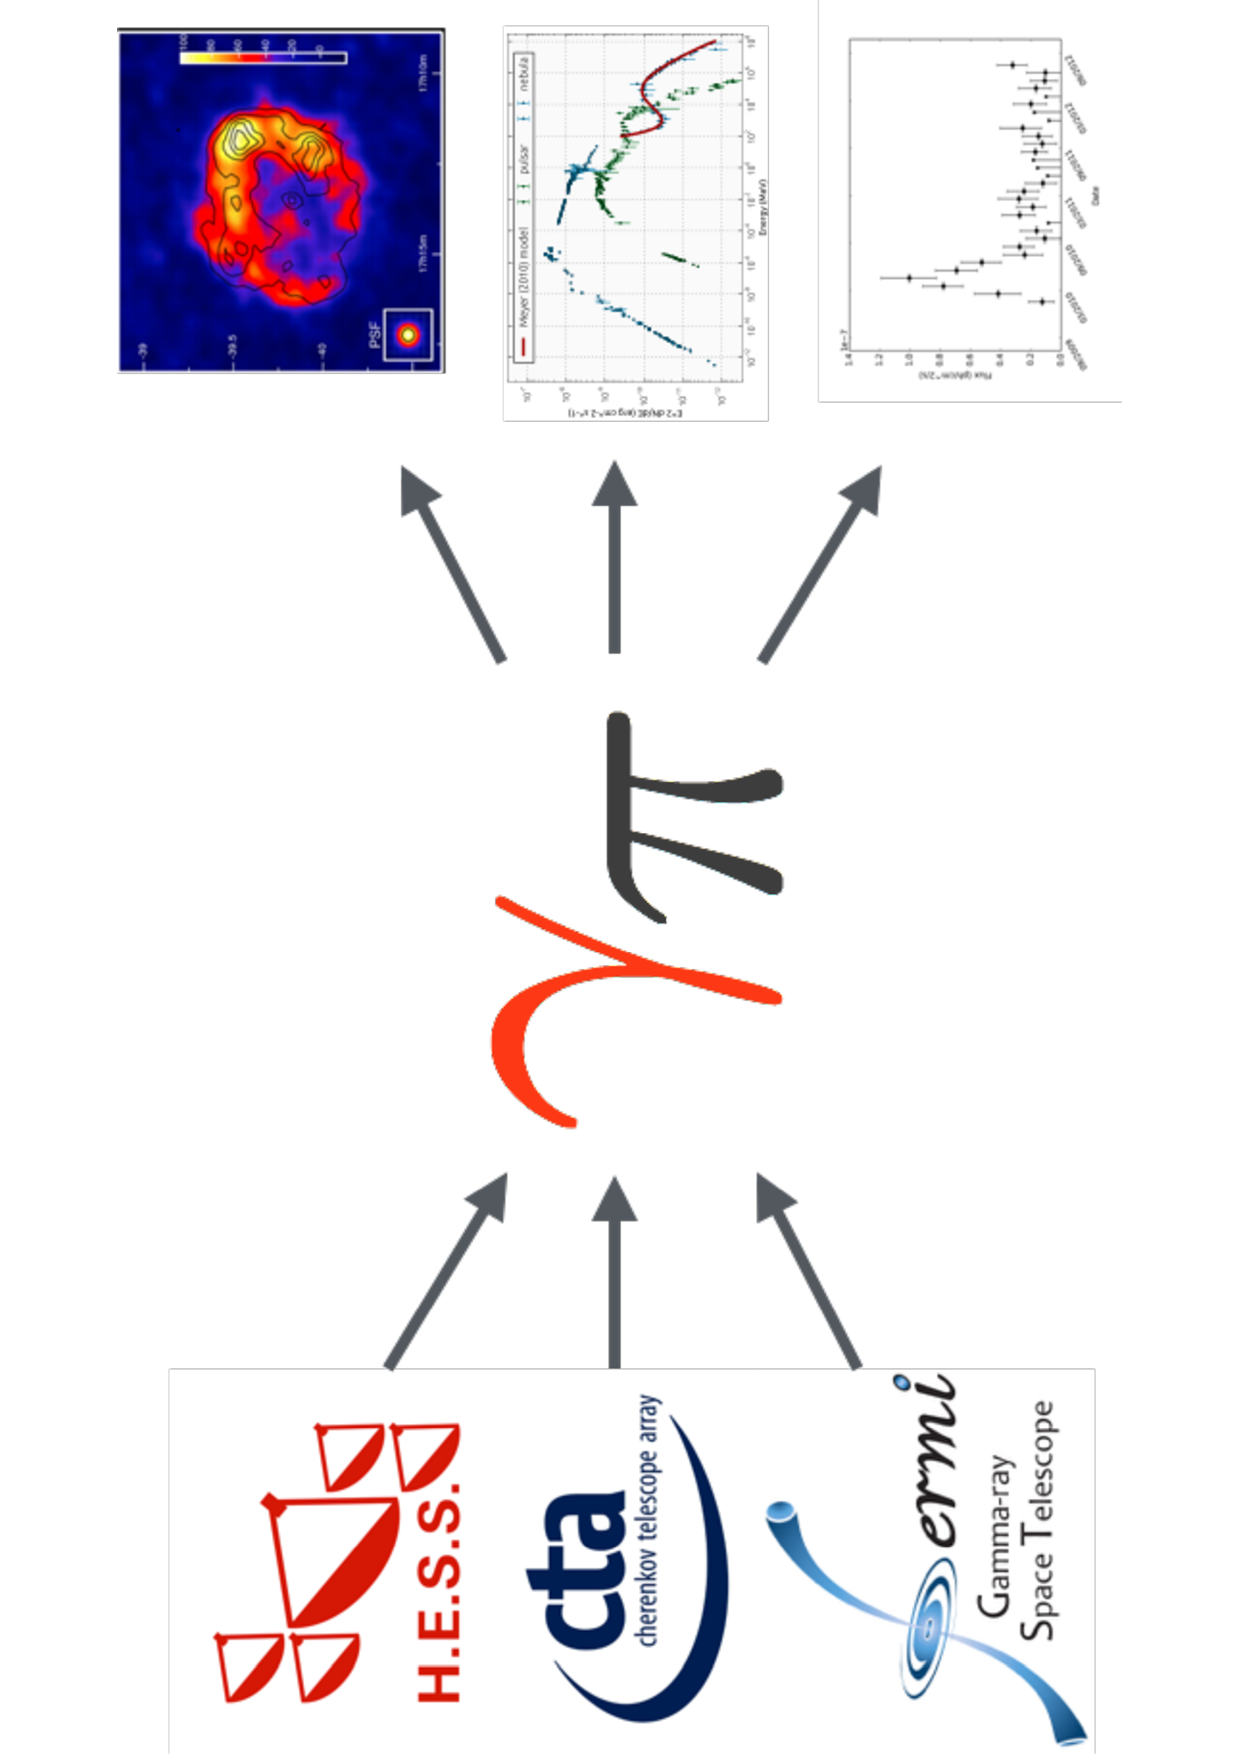
\includegraphics[height=0.5\textwidth, angle=270]{figures/gammapy-big-picture}
\caption{
Gammapy is a Python package for high-level gamma-ray data analysis. Using event
lists, exposures and point spread functions as input you can use it to generate
science results such as images, spectra, light curves or source catalogs. So far
it has been used to simulate and analyse H.E.S.S., CTA and \textit{Fermi}-LAT
data, hopefully it will also be applied to e.g. VERITAS, MAGIC or HAWC data in
the future.
}
\label{fig:big-picture}
\end{figure}

\begin{figure}[t]
\centering
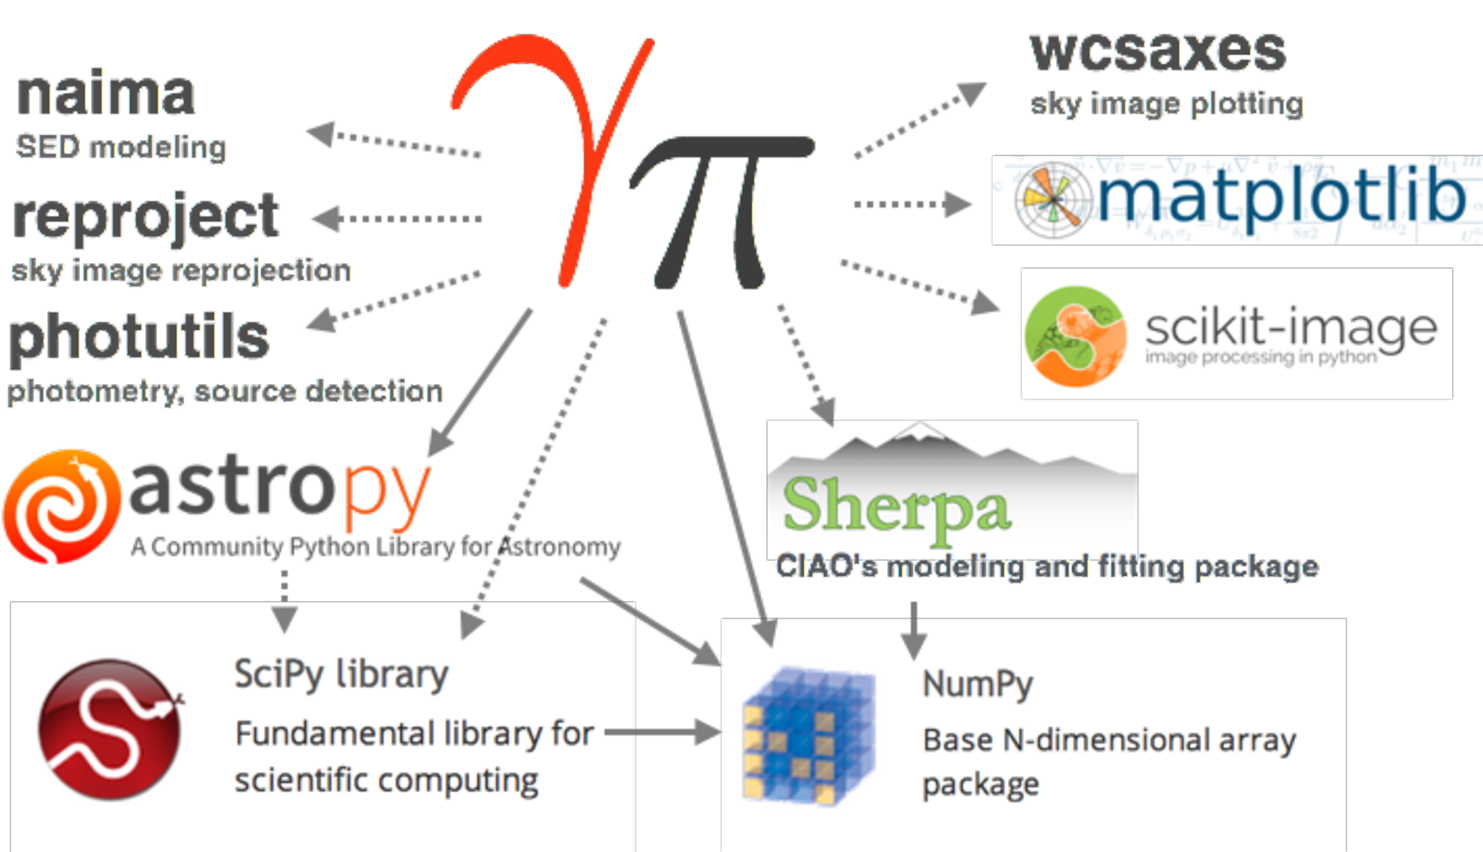
\includegraphics[width=0.5\textwidth]{figures/gammapy-dependencies}
\caption{
The Gammapy stack. Required dependencies Numpy and Astropy are illustrated with
solid arrows, optional dependencies (the rest) with dashed arrows.
}
\label{fig:dependencies}
\end{figure}

\section{Applications}
\label{sec:apps}

\subsection{Source detection}
\label{apps:detect}

See Figure~\ref{fig:fermi-ts-image}.

Ref: \citep{Stewart2009}

\begin{figure*}[t]
\centering
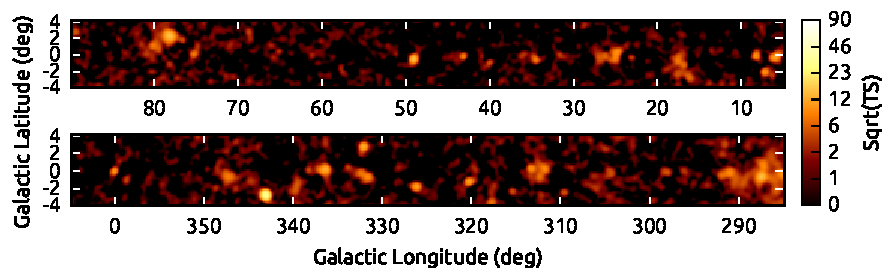
\includegraphics[width=1.\textwidth]{figures/gammapy-fermi-ts-image}
\caption{
Gammapy application example: A \textit{Fermi} survey TS map of the inner
Galactic plane region.
}
\label{fig:fermi-ts-image}
\end{figure*}

\subsection{Morphology analysis}
\label{apps:morph}

\subsection{Spectral analysis}
\label{apps:spec}

\subsection{Cube analysis}
\label{apps:cube}

Maybe. Optional section.

\begin{figure*}[t]
\centering
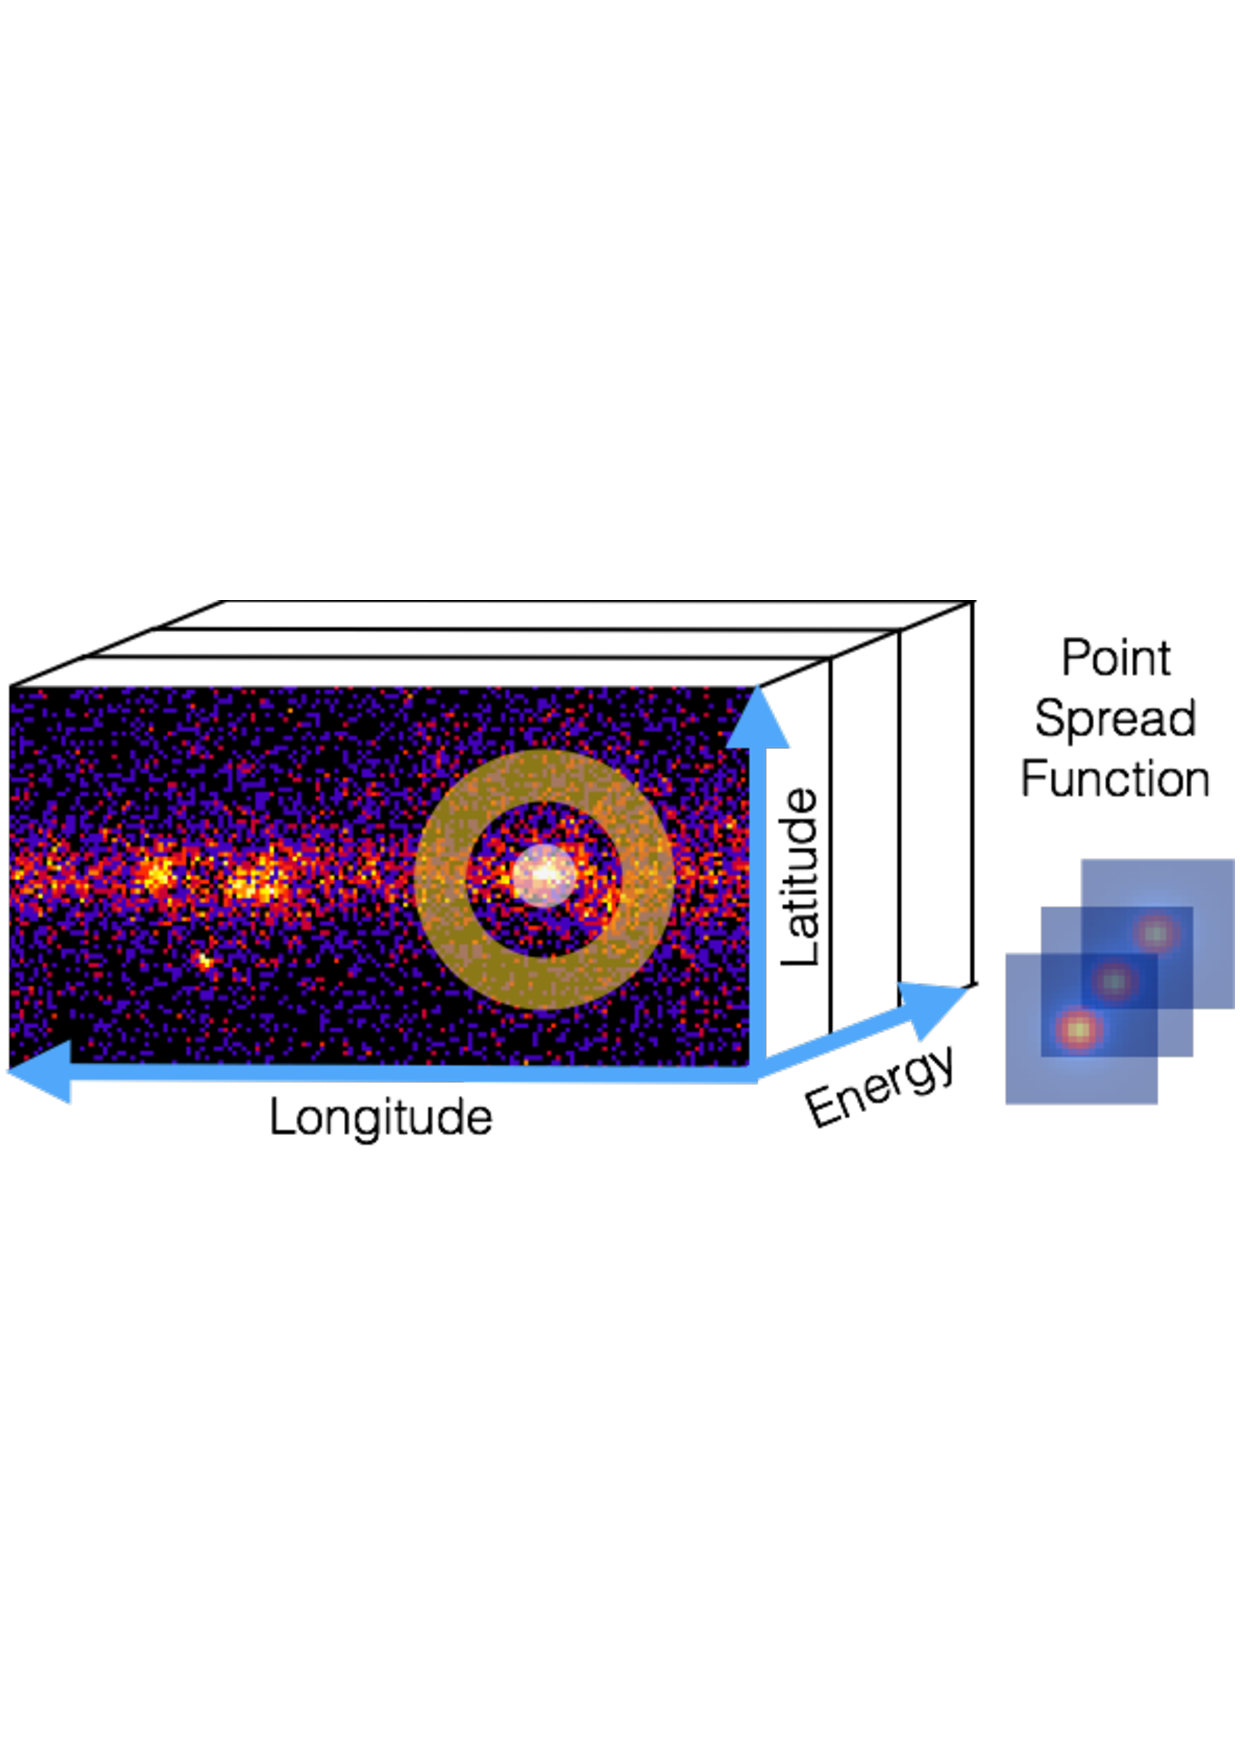
\includegraphics[width=0.8\textwidth]{figures/gammapy-cube-analysis}
\caption{
Gammapy data model illustration. Binned analysis of lon-lat-energy cube data is
supported via joint likelihood analysis of one image per energy bin.
On-off-region based spectral analysis is supported as well.
}
\label{fig:data-model}
\end{figure*}

\subsection{CTA simulation}
\label{apps:sim}

Maybe. Optional section

\section{Development approach}
\label{sec:dev}

\section{Planned functionality}
\label{sec:plans}

\section{Conclusions}
\label{sec:conclusions}

Gammapy is great!

You should try it now!

\begin{acknowledgements}

We would like to thank the \texttt{Numpy}, \texttt{Scipy}, \texttt{IPython} and
\texttt{Matplotlib} communities for providing their packages which are invaluable
to the development of Astropy. We thank the GitHub team for providing us with
an excellent free development platform. We also are grateful to Read the Docs
(\ReadthedocsUrl), and Travis
(\TravisUrl) for providing free documentation
hosting and testing respectively. Finally, we would like to thank all the
Gammapy users that have provided feedback and submitted bug reports.    
    
TODO: copy over stuff from \url{http://docs.gammapy.org/en/latest/about.html#thanks}.

\end{acknowledgements}


% Back matter
\bibliographystyle{aa}
\bibliography{gammapy-paper.bib}

\end{document}
